% Chapter 2

\chapter{Stato dell'arte} % Write in your own chapter title
\label{Capitolo 2}
\lhead{Capitolo 2. \emph{Stato dell'arte}} % Write in your own chapter title to set the page header

\par
In questo capitolo sar\`{a} descritto lo stato dell'arte riguardanti gli studi e le analisi effettuate relative ad informazioni di tipo geolocalizzato riguardanti gli esseri umani; questa tipologia di dati abbraccia diversi ambiti, tra i quali l'ambito sociale e l'ambito scientifico.
\par
L'interesse che gli accademici che si occupano di sociologia e comportamento umano \`{e} dovuto principalmente al modo in cui gli spostamenti delle persone condizionino le amicizie e relazioni tra loro, ma soprattutto come l'analisi dei dati sia spesso contrastante con l'impressione che hanno le persone stesse dei loro spostamenti, come esposto da Nathan Eagle ed altri in \citep{Reference1}.
\par
Un'altro ambito in cui lo studio di informazioni di tipo geolocalizzato \`{e} quello scientifico, dove si pu\`{o} trovare l'applicazione di diverse discipline matematiche per effettuare l'analisi di dati grezzi; tra queste la teoria dei grafi e la statistica sono sicuramente le maggiormente utilizzate. Gli studiosi che si occupano di scienze sono interessati all'aggregazione dei dati grezzi in dati pi� strutturati, per poter, ad esempio, essere in grado di predirre sia le posizioni delle persone nel futuro, sia le relazioni di amicizia tra gli utenti nel tempo.
\\
Infine, utilizzando i dati strutturati in maniera adeguata, \`{e} possibile creare un sistema di raccomandazione e stimare la similitude tra utenti basandosi solamente su informazioni di tipo geolocalizzato.
\newpage
\section{Ambito sociale}
\par
Lo studio di Nathan Eagle ed altri in \citep{Reference1}, il quale � durato complessivamente nove mesi, si basa su 94 soggetti dello stesso gruppo di lavoro dotati di smartphone che hanno installato al loro interno alcune applicazioni che permettono di registrare ed inviare ad i ricercatori diverse informazioni, tra cui il log delle chiamate, l'identificativo dei dispositivi Bluetooth che sono stati a meno di cinque metri dal soggetto e l'identificativo della cella attraverso la quale lo smartphone riceve il segnale.
\par
Oltre a questi dati analitici, che possiamo definire comportamentali, ad ogni soggetto \`{e} stato chiesto di compilare alcuni questionari mensili che mirano a raccogliere informazioni personali riguardanti le relazioni d'amicizia e la durata approssimativa della vicinanza con altri soggetti; i dati emersi da questi questionari vengono definiti autodichiarati.
\par
L'analisi di tutti i dati raccolti � divisa in tre fasi:
\begin{itemize}
  \item analisi della relazione tra dati comportamentali ed autodichiarati
  \item analisi della presenza di dati comportamentali che caratterizzano l'amicizia
\end{itemize}

\subsection{Relazione tra dati comportamentali ed autodichiarati}
Negli ultimi trent'anni si \`{e} discusso molto sull'affidabilit\`{a} delle misurazioni esistenti per le relazioni, osservando soprattutto che le osservazioni comportamentali sono debolmente correlate con le interazioni riportate dai soggetti; alcuni studi \citep{Reference2} hanno dimostrato come le persone riescono a ricordare meglio le strutture sociali a lungo termine rispetto a quelle nel breve periodo. Si possono riscontrare due diverse tipologie di bias, uno basato sul ricordo degli eventi recenti denominato \emph{recency bias}, l'altro basato sul ricordo degli eventi pi� importanti denominato \emph{salience bias}; attraverso i dati raccolti si pu� quindi assimilare l'effetto di \emph{recency bias} alla quantit�\`{a} di interazioni in un periodo prefissato antecedente al questionario e l'effetto di \emph{salience bias} alla presenza o meno di una relazione di amicizia tra due soggetti.
\par
Attraverso l'incrocio dei dati comportamentali ed autodichiarati \`{e} emerso che la maggiorparte della prossimit� \`{e} misurata \`{e} stata invece dichiarata dal soggetto come non vicinanza; inoltre, quando i due dati non erano in contrasto, il tempo di contatto � sempre stato sovrastimato, essendo la media dei dati comportamentali di 33 minuti al giorno contro la media dei dati autodichiarati di 87 minuti al giorno. Infine si \`{e} osservato che i dati riportati da soggetti che si reputano amici sono molto pi� precisi rispetto ai dati riportati da soggetti che non si considerano amici.

\subsection{Analisi della presenza di dati comportamentali che caratterizzano l'amicizia}
Analizzare i dati comportamentali per evidenziare il grado di relazioni tra due soggetti, come l'amicizia, \`{e} diverso da misurarne la vicinanza; infatti \`{e} plausibile che due persone anche essendo amiche, siano distanti anche per periodi di tempo piuttosto lunghi. Ad ogni modo il contesto, sia spaziale che temporale, pu� aiutare a definire alcuni pattern per la predizione delle amicizie, ad esempio l'aver passato con un'altra persona poche ore un sabato sera in un posto diverso dal luogo di lavoro indica una relazione differente rispetto all'aver passato quattro ore nel luogo di lavoro di un mercoled\`{i} pomeriggio.
\par
In figura ~\ref{fig:Proximity} \`{e} rappresentata graficamente la distribuzione della probabilit� di vicinanza sia all'interno del luogo di lavoro, sia all'esterno, tra persone che si reputano amici reciprocamente, persone tra le quali solamente una delle parti si reputa amica dell'altra parte e persone che non si reputano amici a vicenda; si nota immediatamente come la vicinanza \`{e} pi� probabile tra le prime due categorie di persone, ma, essendo il luogo d'incontro un fattore determinante, si pu\`{o} osservare come la vicinanza misurata all'esterno del luogo di lavoro sia maggiore per chi si reputa amico reciprocamente.

\begin{figure}[htbp]
  \centering
    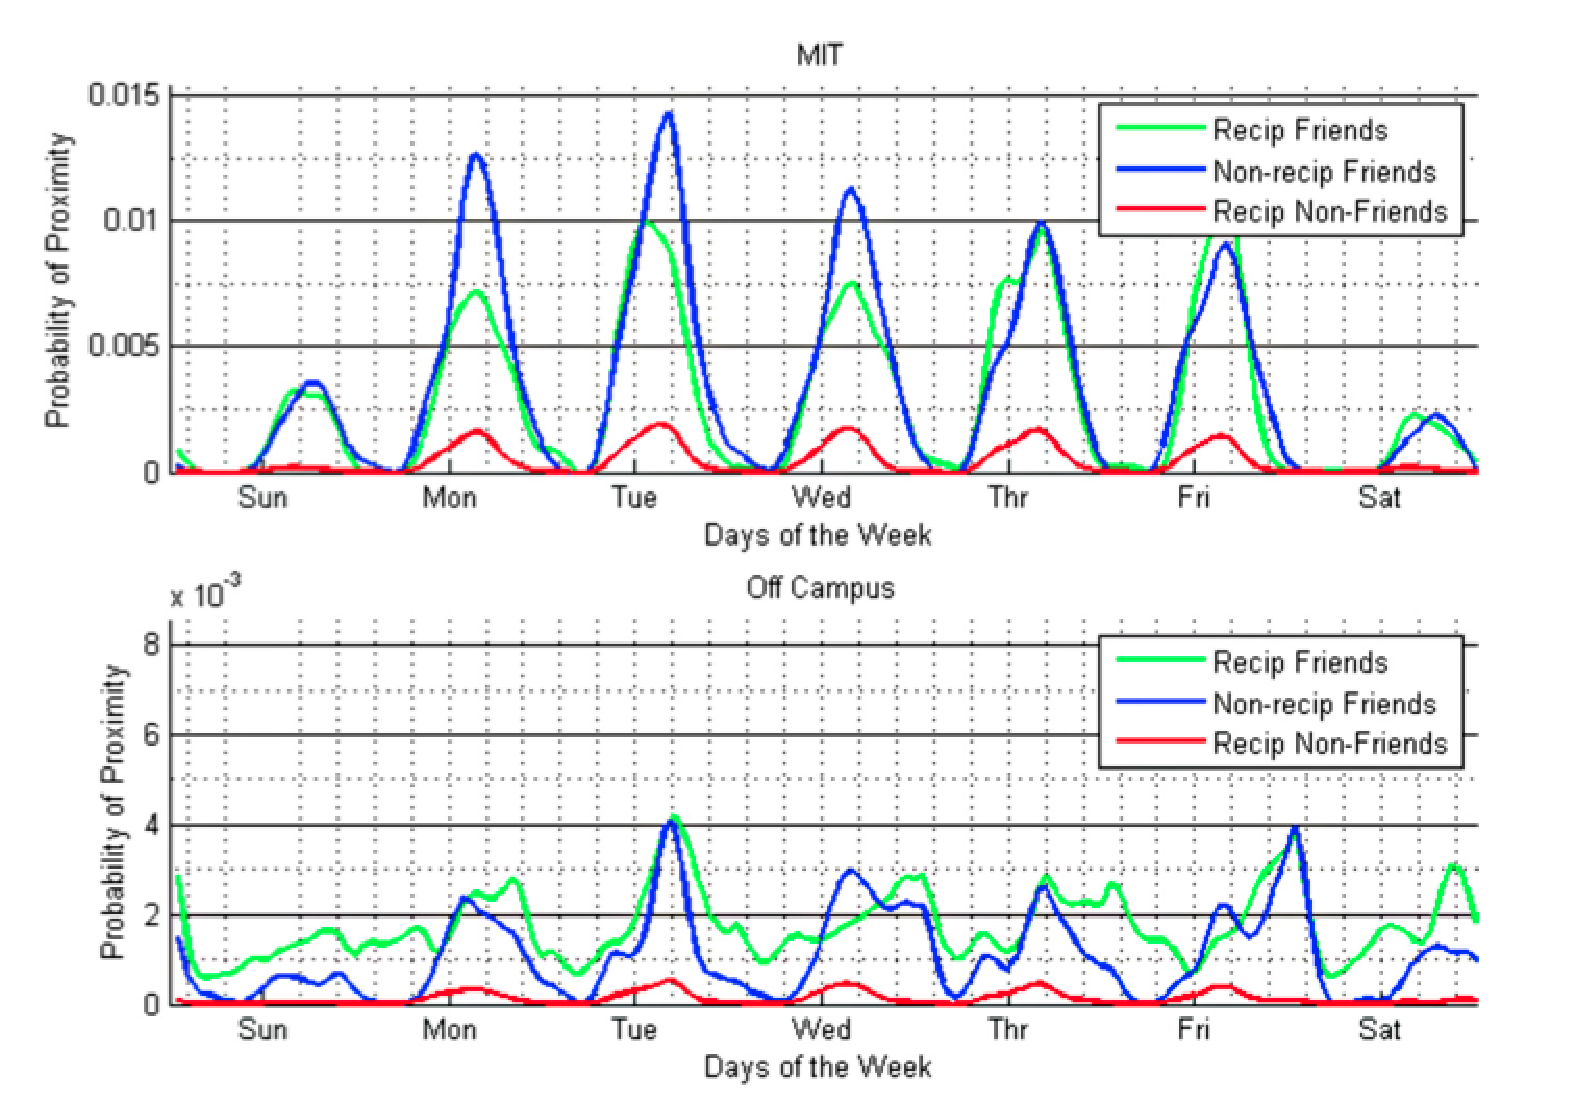
\includegraphics[width=0.8\textwidth]{./Figures/nathan_1.pdf}
    \rule{35em}{0.5pt}
  \caption[Distrubuzione della vicinanza]{Distribuzione della vicinanza nel tempo e nello spazio}
  \label{fig:Proximity}
\end{figure}

Nathan Eagle ed altri hanno successivamente classificato la vicinanza in diverse variabili corrispondenti alla vicinanza all'interno o all'esterno del campus, alla vicinanza di giorno o di notte e alla vicinanza nei giorni lavorativi o nei fine settimana; una fattorizzazione di queste variabili ha evidenziato come esistano solamente due fattori discriminanti, ovvero la vicinanza durante le ore del giorno nel luogo di lavoro e la vicinanza nelle ore serali o nei fine settimana all'esterno del campus. Solamente utilizzando il secondo fattore \`{e} possibile predirre il 96\% percento dei rapporti di non amicizia reciproca ed il 95\% percento dei rapporti di amicizia reciproca, potendo quindi tralasciare i dati autodichiarati di amicizia, quest'ultima risulta stimabile correttamente utilizzando solamente i dati comportamentali.


\section{Ambito scientifico}
\subsection{Predizione delle traiettorie}

\subsection{Similitude tra utenti}
Negli ultimi anni gli utenti del web hanno iniziato ad utilizzare tecnologie per il tracciamento dei dati GPS anche per registrare esperienze sportive o viaggi personali, per poi condividerle nel web con altri utenti oppure per visualizzare in una mappa i propri spostamenti. Tuttavia le applicazioni che utilizzano i tracciati GPS utilizzano i dati grezzi, senza focalizzarsi sulla comprensione degli stessi; esistono inoltre applicazioni che cercano di razionalizzare i log derivati dal tracciamento GPS, estrapolando l'attivit\`{a} che un utente sta compiendo in quel momento, come ad esempio una corsa a piedi o in bicicletta, oppure cercando di sintetizzare i dati grezzi in luoghi che un utente ha visitato.
\par
Un ulteriore campo di applicazione che prevede l'utilizzo di tracciati GPS riguarda il confronto tra diversi utenti per calcolare la similitudine tra essi, come hanno provato ad analizzare Quannan Li ed altri in \citep{Reference6}. Secondo la prima legge della geografia ogni cosa \`{e} correlata, ma le cose che sono pi\`{u} vicine in termini geografici lo sono di pi\`{u}, quindi la tesi dei ricercatori, basandosi su questa legge, consiste nella similitudine tra due utenti in base alla loro storia in termini di tracciati GPS.
\subsubsection{Definizioni}
\begin{description}
  \item[Log Gps]: Un log GPS \`{e} una sequenza di punti GPS, che contengono una coordinata che rappresenta la latitudine, una coordinata che rappresenta la longitudine ed il timestamp della registrazione.
  \item[Punto stazionario]: Un punto stazionario \`{e} una regione geografica dove l'utente rimane per un determinato periodo ti tempo; a differenza di un punto GPS, un punto stazionario possiede un significato semantico, come ad esempio la casa o l'ufficio, 
  \item[Storia dei luoghi]: Dato un log GPS e i punti stazionari che si possono ricavare, la storia dei luoghi di un utente \`{e} rappresentata dalla sequenza dei posti che esso ha visitato, corredati di una data di arrivo ed una data di partenza.
  	\item[Grafo gerarchico]: La similitudine in termini geografici tra due utenti non \`{e} binaria, ma deve essere valutata rispetto ad una scala; per questo motivo i ricercatori hanno considerato l'insieme di tutti i punti stazionari di tutti gli utenti come un unico dataset che hanno poi clusterizzato utilizzando la distanza tra i vari punti stazionari; ad ogni step dell'algoritmo di clusterizzazione veniva generato un nuovo livello in cui i cluster rappresentavano aree geografiche pi� ampie. Ad ogni livello hanno potuto creare dei grafi diretti per ogni utente, in cui un nodo era rappresentato dal cluster di appartenenza del punto stazionario del relativo utente, mentre un arco veniva tracciato tra due cluster quando la traiettoria dell'utente cambiava area geografica; in questo modo la similitudine tra due utenti \`{e} pu\`{o} essere valutata per ogni livello sulla base dei cluster e delle traiettorie tra cluster condivise, risultando in una similitudine pi\`{u} elevata per le condivisioni che avvengono ai livelli pi\`{u} bassi. Questo procedimento \`{e} illustrato in \ref{fig:hirarchical_graph}. 
\end{description}

\begin{figure}[htbp]
  \centering
    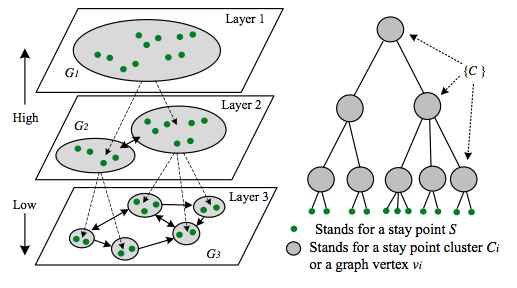
\includegraphics[width=0.8\textwidth]{./Figures/hierarchical_graph.png}
    \rule{35em}{0.5pt}
  \caption[Grafo gerarchico]{Rappresentazione del grafo gerarchico basato su cluster di punti stazionari}
  \label{fig:hirarchical_graph}
\end{figure}

\subsubsection{Processo per il calcolo della similitudine}
La struttura del grafo gerarchico di \ref{fig:hirarchical_graph} \`{e} una valida rappresentazione della storia dei luoghi di un utente, contenente quindi sia informazioni di tipo spaziale che temporale; i ricercatori, per poter calcolare la similitudine tra due utenti, hanno innanzitutto cercato i nodi in comune nei rispettivi grafi gerarchici degli utenti e successivamente sono state generate delle sequenze contenenti i nodi trovati, riconducendo il problema della similitudine di due utenti ad un problema di pattern matching tra sequenze di oggetti.

\begin{figure}[htbp]
  \centering
    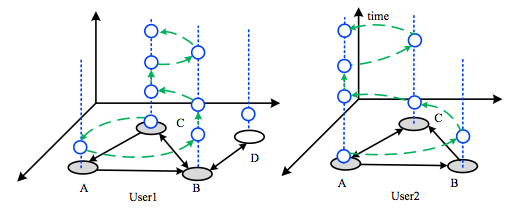
\includegraphics[width=0.8\textwidth]{./Figures/sequence_rapresentation.png}
    \rule{35em}{0.5pt}
  \caption[Rappresentazione delle sequenze]{Rappresentazione delle sequenze di due utenti}
  \label{fig:sequence_rapresentation}
\end{figure}

In \ref{fig:sequence_rapresentation} sono visualizzati due grafi gerarchici di due utenti distinti allora stesso livello di clusterizzazione; in ognuno dei due grafi sono tracciati in grigio i nodi che corrispondono al cluster, mentre i nodi pi\`{u} colorati in blu e collegati con una linea tratteggiata identificano i punti stazionari visitati dagli utenti in tempi diversi. La freccia tratteggiata in verde, invece, rappresenta la successione temporale in cui gli utenti hanno esplorato i propri punti stazionari.
\par
Si pu\`{o} notare come i due utenti condividano i nodi $A$, $B$ e $C$ e generino, rispettivamente, le sequenze $<C, A, B, B, C, C, B, C>$ e $<A, B, C, A, A, C, A>$ che per semplicit\`{a} vengono rappresentate con $<C(1), A(1), B(2), C(2), B(1), C(1)>$ e  $<A(1), B(1), C(1), A(2), C(1), A(1)>$ dove il numero tra parentesi che segue il nome di un nodo rappresenta il numero di volte che un utente ha viaggiato successivamente in punti stazionari appartenenti allo stesso cluster; utilizzando inoltre il tempo di entrata e di uscita da ogni cluster \`{e} possibile calcolare l'intervallo di tempo $\Delta t_I$ tra due elmetti delle sequenze, ottenendo:
\par
	User 1: $C(1) \xrightarrow{\Delta t_1} A(1) \xrightarrow{\Delta t_2} B(2) \xrightarrow{\Delta t_3} C(2) \xrightarrow{\Delta t_4} B(1) \xrightarrow{\Delta t_5} C(1)$ \\
	User 2: $A(1) \xrightarrow{\Delta t_{1'}} B(1) \xrightarrow{\Delta t_{2'}} C(1) \xrightarrow{\Delta t_{3'}} A(2) \xrightarrow{\Delta t_{4'}}  C(1) \xrightarrow{\Delta t_{5'}}  A(1)$
\par
In modo generico, quindi, la storia dei luoghi di un utente pu\`{o} essere scritta come:
\begin{center}
	$seq=<a_1(k_1) \xrightarrow{\Delta t_1} a_2(k_2) \xrightarrow{\Delta t_2} a_3(k_3) \xrightarrow{\Delta t_3} \ldots >$
\end{center}
dove $a_i \in V$ \`{e} l'identificativo del cluster e $k_i$ \`{e} il numero di volte che un utente ha visitato successivamente un punto stazionario all'interno del cluster $a_i$. In modo analogo si pu\`{o} calcolare il tempo tra due elementi della sequenza come:
\begin{center}
	$\Delta t_i = a_{i+1}(0).arvT - a_i(k_i - 1).levT $
\end{center}
dove $arvT$ identifica il tempo di entrata, $levT$ il tempo di uscita e l'indice all'interno delle parentesi tonda identifica un punto stazionario all'interno del cluster.

\paragraph{Pattern matching}
Per definire simili due sequenze devono essere soddisfatte le seguenti condizioni:
\begin{center}
	$seq_1=<a_1(k_1) \xrightarrow{\Delta t_1} a_2(k_2) \xrightarrow{\Delta t_2} a_3(k_3) \xrightarrow{\Delta t_3} \ldots a_m(k_m)>$ \\
	$seq_2=<b_1(k_{1'}) \xrightarrow{\Delta t_{1'}} b_2(k_{2'}) \xrightarrow{\Delta t_{2'}} b_3(k_{3'}) \xrightarrow{\Delta t_{3'}} \ldots b_m(k_{m}')>$
\end{center}
\begin{enumerate}
  \item $\forall 1 \le i \le m, a_i = b_i$, ovvero i nodi alla stessa posizione devono avere lo stesso identificativo.
  \item $\forall 1 \le i < m, |{\Delta t_i - \Delta t_{i'}}| \le t_{th}$, ovvero due utenti devono avere un'intervallo di tempo tra due transizioni minore di una certa soglia. 
  
\end{enumerate}
Utilizzando questa definizione di similitudine tra due sequenze \`{e} possibile definire sequenze simili di lunghezza diversa; un esempio di queste definizione si pu\`{o} visualizzare graficamente in \ref{fig:m_lenght}
\par
Per calcolare la similitudine tra due utenti, basandosi sulle definizione precedentemente date, si dovranno tener conto sia delle lunghezze delle diverse sequenze simili tra loro ma anche del livello del grafo gerarchico in cui queste sequenze sono state calcolate; possiamo quindi definire il punteggio di ogni sequenza come:
\begin{center}
	$ s_{(m)} = \alpha_{(m)}\sum_{i=1}^{m} min(k_i,k_{i'})$
\end{center}
dove $\alpha_{(m)}$ \`{e} un coefficiente che dipende dalla lunghezza $m$ della sequenza e che aumenta il punteggio per le sequenze pi\`{u} lunghe.
\par
La similitude di due utenti ad un certo livello del grafo gerarchico si basa invece su tutte le sequenze simili trovate in quel livello; si pu\`{o} quindi definire:
\begin{center}
	$ S_t = \frac{1}{N_1 * N_2} \sum_{i = 1}^{n} s_i$
\end{center}
dove $s_i$ \`{e} il punteggio della sequenza i-esima calcolata con la formula precedente, $n$ \`{e} il numero di sequenze simili tra due utenti trovati nello specifico livello ed $N_1$ e $N_2$ sono rispettivamente il numero di punti stazionari dei due utenti. La divisione per questi due fattori \`{e} motivata da un problema di bilanciamento tra i dati di due utenti; intuitivamente se non venisse tenuto conto della quantit\`{a} di dati gli utenti che hanno maggior punti stazionari sarebbero favoriti nel contenere al loro interno sequenze simili di coloro che hanno meno punti stazionari.
\par
Infine i ricercatori hanno definito una misura di similitudine tra utenti attraverso tutti i livelli, definita come la somma pesata attraverso un opportuno coefficiente dipendente dal livello, che a livelli inferiori assume un valore maggiore, di tutti i vari punteggi ottenuti sui livelli del grafo gerarchico.

\begin{figure}[htbp]
  \centering
    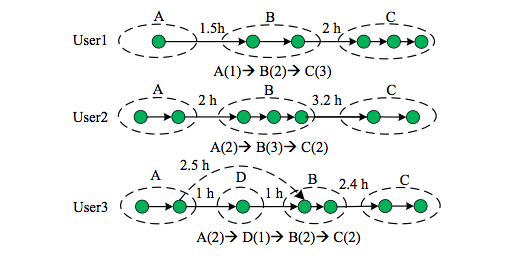
\includegraphics[width=0.8\textwidth]{./Figures/m_length.png}
    \rule{35em}{0.5pt}
  \caption[Sequenze simili]{Similitudine tra sequenze tra tre utenti}
  \label{fig:m_lenght}
\end{figure}

\subsection{Sistema di raccomandazione}
Un sistema di raccomandazione \`{e} una soluzione che cerca di predirre una valutazione o un insieme di preferenze che un utente attribuirebbe ad un oggetto; esistono diverse metodologie per la costruzione e l'applicazione di un tale sistema divisibili in due categorie principali:
\begin{itemize}
	\item collaborative filtering
	\item content-based filtering
\end{itemize}
\subsubsection{Collaborative filtering}
L'approccio di tipo \emph{collaborative filtering} si basa essenzialmente sul collezionare ed analizzare un grande numero di informazioni sui comportamenti, sulle attivit\`{a} o sulle preferenze degli utenti e di predirre successivamente quello che pu\`{o} interessare ad un utente basandosi sulla similitudine con altri utenti; uno dei principali vantaggi di questa soluzione risiede nel fatto che non \`{e} necessario che i contenuti da proporre siano ``capibili'' dalla macchina, potendo quindi raccomandare elementi complessi quali film, musica o libri.
\par
La raccolta delle preferenze degli utenti pu\`{o} essere effettuata in due modalit\`{a}, spesso utilizzate congiuntamente, ovvero la raccolta di dati espliciti da parte degli utenti, come ad esempio chiedere all'utente di valutare un oggetto o di scegliere tra due oggetti quali preferisce, e la raccolta di dati impliciti, come ad esempio osservare gli oggetti che un utente visita in un sito di e-commerce oppure memorizzare una lista degli ultimi oggetti acquistati.
La similitudine tra gli utenti, invece, viene valutata utilizzando spesso tecniche che appartengono a diverse discipline, come l'algoritmo k-NN per la classificazione di elementi derivato dal \emph{machine learning} oppure come la correlazione di Pearson derivata dalla statistica. 
\par
Molti sono i sistemi di \emph{collaborative filtering} presenti, sia commerciali che non commerciali, tra cui i pi\`{u} famosi comprendono il sistema di Amazon.com che propone oggetti che altri utenti hanno acquistato congiuntamente all'oggetto che si desidera acquistare in quel momento, Last.fm che consiglia un brano musicale basandosi sulle abitudini d'ascolto di altri utenti e Facebook che consiglia nuovi possibili amici basandosi sulle connessione tra gli utenti ed i loro amici.
\par
Questo tipo di approccio soffre di alcuni problemi, tra cui i principali si possono riassumere in:
\begin{itemize}
	\item Cold Start: questi sistemi richiedono un'enorme quantit\`{a} di dati presente per ogni utente per poter generare raccomandazioni accurate.
	\item Scalability: nella maggiorparte dei sistemi di raccomandazioni esistono milioni di utenti ed oggetti, necessitando quindi di una grande potenza di calcolo.
	\item Sparsity: il numero di oggetti che un utente pu\`{o} valutare \`{e} spesso elevato, quindi \`{e} molto probabile che per ogni oggetto ci siano poche valutazioni da parte degli utenti, anche per l'oggetto che ad esempio ha pi\`{u} vendite in un sito di e-commerce.
\end{itemize}

\subsubsection{Content-based filtering}
Un'altro approccio comune tra i sistemi di raccomandazione \`{e} il \emph{content-based filtering} che si basa sulle descrizione degli oggetti e sul profili delle preferenze degli utenti; in questo tipo di sistema, le parole chiave sono utilizzate per descrivere gli oggetti, mentre i profili delle preferenze degli utenti sono costruite per indicare che tipologia di oggetti l'utente predilige. 
\par
Il confronto tra le preferenze degli utenti e le descrizioni degli oggetti \`{e} effettuato utilizzando algoritmi di information retrieval basati sugli spazi vettoriali; il sistema scompone le descrizioni degli oggetti in un insieme di attributi discreti che possono essere rappresentati quindi come vettori in modo analogo a come accade per i documenti in un sistema di information retrieval, mentre il profilo dell'utente rappresenta la query di ricerca. Come accade nei sistemi di information retrieval classici, diverse tecniche possono essere utilizzate sia per determinare la rilevanza di un oggetto nei confronti di un utente, tra cui BM25 o le reti neurali, sia per validare e migliorare l'efficacia dell'algoritmo a posteriori proponendo all'utente di valutare l'oggetto reperito dal sistema.
\par
Uno tra i pi\`{u} noti sistemi di raccomandazione basati sul \emph{content-based filtering} \`{e} utilizzato da Pandora Radio, che permette ad un utente di ascolta musica con caratteristiche simili ad una canzone che l'utente ha inviato precedentemente e che quindi sar\`{a} utilizzata come query di ricerca.

\subsubsection{Location-content-aware filtering}
L'emergere di social network sia basati sugli eventi, come Meetup e DoubanEvent, sia basati sulla posizione geografica, come Foursquare o Gowalla, hanno permesso a Hongzhi Yin ed altri\citep{Reference3} di sperimentare un nuovo sistema di raccomandazione basato su dati geolocalizzati per predirre posti o eventi agli utenti basandosi sugli interessi personali e sulle preferenze locali, ovvero l'insieme delle preferenze degli utenti in una determinata area.
\par
La realizzazione di un tale sistema comprende ulteriori difficolt\`{a} rispetto ai precedenti, in quanto una persona difficilmente visita molti luoghi diversi, causando quindi una grande sparsit\`{a} nella matrice utenti-posti; inoltre \`{e} molto frequente che un utente visiti posti od eventi in un'area circoscritta alla citt\`{a} in cui vive, rendendo quindi molto difficile il suggerimento di buone raccomandazioni in citt\`{a} diverse, data la mancanza di dati storici per quell'utente. Alcune analisi infatti evidenziano come le attivit\`{a} che un utente compie all'esterno dell'area della propria citt\`{a} rappresentino solamente lo 0.47\% delle attivit\`{a} complessive, introducendo quindi il problema denominato della \emph{new city}.
\par
Un esempio che rafforza l'intenzione degli autori di creare un nuovo sistema di raccomandazione per questa tipologia di dati pu\`{o} essere il seguente: un utente $u$ \`{e} uno shopaholic e tende a visitare spesso il centro commerciale $v^`$ nella sua citt\`{a}; $v$ \`{e} un centro commerciale molto popolare nella citt\`{a} $l_v$ di cui $u$ \`{e} nuovo. Intuitivamente un buon sistema di raccomandazione suggerirebbe $v$ ad $u$ quando quest'ultimo di trova ad $l_v$, ma un metodo basato sul \emph{collaborative filtering} fallirebbe in quanto ci sarebbero troppi pochi utenti in comune tra $v$ e $v^`$ e di conseguenza i vettori di $v$ e $v^`$ non sarebbero simili.
\par
Il sistema di raccomandazione creato da Hongzhi Yin ed altri si basa su due modelli, uno offline ed uno online, come rappresentato in ~\ref{fig:OfflineOnline}.

\begin{figure}[htbp]
  \centering
    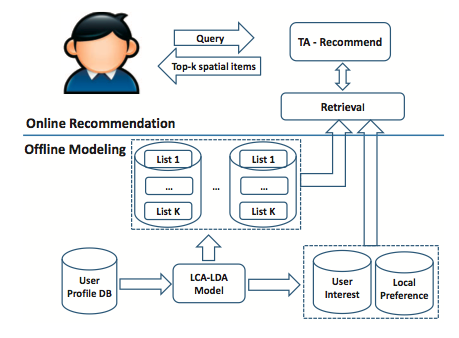
\includegraphics[width=0.8\textwidth]{./Figures/offline_online.png}
    \rule{35em}{0.5pt}
  \caption[Online ed offline]{Rappresentazione del sistema di raccomandazione di Hongzhi Yin ed altri}
  \label{fig:OfflineOnline}
\end{figure}

\paragraph{Modello offline}
Il modello offline, denominato LCA-LDA, \`{e} un modello generativo basato sulla probabili\`{a} che cerca di simulare il processo di decisione umano nella scelta di posti ed eventi; questo modello considera sia gli interessi personali dell'utente, sia le preferenze locali in maniera unificata con la seguente formula:
\begin{center}
$P(v | \theta_u,\theta_{l_u}) = \lambda_uP(v | \theta_u) + (1 - \lambda_u)P(v | \theta_{l_u})$
\end{center}
dove $P(v | \theta_u)$ \`{e} la probabilit\`{a} che il posto $v$ sia generato secondo gli interessi personali dell'utente $u$, indicati con $\theta_u$m e $P(v | \theta_{l_u})$ \`{e} la probabilit\`{a} che l'elemento $v$ sia generato secondo le preferenze locali, indicate con $\theta_{l_u}$. Il parametro $\lambda_u$ \`{e} un moltiplicatore che quantifica l'influenza degli interessi personali rispetto alle preferenze locali per l'utente $u$.
\par
I valori dei parametri nascosti, ovvero $\theta_u$, $\theta_{l_u}$ e $ \lambda_u$ sono inferiti utilizzando diverse iterazione del campionamento di Gibbs
\paragraph{Modello online}
Una query nel sistema di raccomandazione presentato \`{e} composta da due argomenti $(u, l_u)$, ovvero un utente $u$ con una citt\`{a} $l_u$ dove desidera viaggiare. Il risultato \`{e} una lista di posti o eventi della citt\`{a} $l_u$ ordinati secondo la probabilit\`{a} calcolata nel modello offline. Durante l'interrogazione \`{e} necessario calcolare il punteggio per ogni posto o evento e successivamente selezionare i miglio $k$ risultati; quando il numero di posti o eventi diventa molto grande, ad esempio supera il milione, il calcolo dei primi $k$ elementi richiede milioni di operazioni tra vettori.
\par
Per migliorare il tempo di calcolo necessario i ricercatori hanno esteso l'algoritmo basato sulle soglie descritto in \citep{Reference4} cercando di mantenere offline una lista dei posti o degli eventi ordinati per le preferenze locali; in questo modo \`{e} sufficiente solamente calcolare le probabilit\`{a} per gli interessi specifici degli utenti.

\paragraph{Dataset utilizzato}
DoubanEvent \`{e} il pi\`{i} grande social network sugli eventi in Cina, dove un utente pu\`{o} creare un evento specificando cosa, dove e quando l'evento si terr\`{a}; successivamente gli altri utenti possono esprimere il loro intento a partecipare o meno all'evento creato. Il dataset utilizzato nell'esperimento di Hongzhi Yin ed altri \`{e} estratto da DoubanEvent e contiene 100.000 utenti, 300.000 eventi e 3.500.000 espressioni di partecipazione da parte degli utenti.

\paragraph{Risultati ottenuti}
Per validare i risultati ottenuti, i ricercatori hanno confrontato la \emph{recall} dei primi $k$ risultati sia in query che contenevano la citt\`{a} propria dell'utente, sia in query che contenevano nuove citt\`{a}. In ~\ref{fig:lcars_result} si pu\`{o} notare come il sistema LCA-LDA proposto sia migliore sia nella raccomandazione di posti o eventi nella citt\`{a} di appartenenza dell'utente, sia nel risolvere il problema della \emph{new city}, mostrando una recall di 0.33@10 e di 0.42@20.

\begin{figure}[htbp]
  \centering
    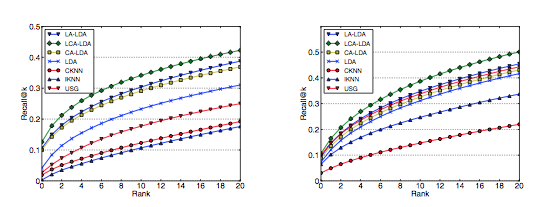
\includegraphics[width=0.8\textwidth]{./Figures/lcars_result.png}
    \rule{35em}{0.5pt}
  \caption[Recall@k]{Risultati della recall@k nelle nuove citt\`{a} (a sx) e nella citt� propria dell'utente (a dx)}
  \label{fig:lcars_result}
\end{figure}

\subsection{Predizione delle connessioni tra utenti}
Il suggerimento di nuovi amici nei social network utilizza principalmente le relazioni di amicizia tra gli utenti ed i loro amici; con l'introduzione di servizi di geolocalizzazione, quali Facebook Places o Foursquare, le informazioni finora utilizzate possono essere ampliate aggiungendo i posti frequentati dagli utenti. Una caratteristica fondamentale di social network basati sulla posizione geografica consiste nella presenza di milioni di nodi, ma allo stesso tempo una grande sparsit\`{a}, risultando in una bassa densit\`{a} di archi tra i vari nodi.
\par
Salvatore Scellato ed altri \citep{Reference5} hanno cercato di utilizzare questa nuova tipologia di informazioni per rispondere alla domanda: \emph{Com'\`{e} possibile progettare un sistema di predizione dei collegamenti tra utenti utilizzando i loro check-in?}. Infatti in questi sistemi le interazioni che gli utenti hanno con i luoghi \`{e} volontario, ovvero un utente deve effettuare una specifica azione, come ad esempio il click su di un link, per poter registrare la propria posizione presso quel luogo; tale azione \`{e} denominata check-in.


\begin{figure}[htbp]
  \centering
    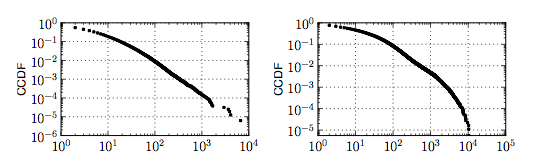
\includegraphics[width=0.8\textwidth]{./Figures/gowalla_ccdf.png}
    \rule{35em}{0.5pt}
  \caption[Distribuzione delle amicizie e dei luoghi del mese di Agosto]{CCDF del numero di amici (a sx) e del numero di luoghi (a dx) per utente}
  \label{fig:gowalla_ccdf}
\end{figure}

\subsubsection{Dataset utilizzato}
Gowalla \`{e} un servizio di social network creato nel 2008 e permette agli utenti di aggiungere amici e condividere la propria posizione; la relazione di amici \`{e} reciproca, ovvero ogni utente deve accettare la relazione di amicizia per perch\`{e} sia permessa la condivisione della posizione. I ricercatori hanno scaricato quattro snapshot mensili da Gowalla, tra maggio e agosto del 2010, riassunti in \ref{table:gowalla} dove \`{e} possibile notare come il numero di utenti registrati e salito da circa 250 mila a circa 380 mila, risultando per\`{o} invariata la percentuale di utenti attivi, ovvero coloro che hanno almeno un check-in o un amico.
\par

\begin{table}
\begin{center}
\begin{tabular}{| c | c | c | c | c |}
\hline
 Mese & Utenti & Utenti attivi & Luoghi & Check-in \\ \hline
 Maggio & 252.000 & 148.234 & 958.823 & 7.475.401 \\
 Giugno & 291.812 & 168.925 & 1,104.771 & 9.073.157 \\
 Luglio & 325.025 & 189.512 & 1.226.847 & 10.537.516 \\
 Agosto & 382.750 & 216.734 & 1.421.262 & 12.846.151 \\
 \hline
\end{tabular}
\caption{Snapshot Gowalla tra maggio e agosto 2010}
\label{table:gowalla}
\end{center}
\end{table}

In \ref{table:gowalla_graph}, invece, sono descritte le propriet\`{a} del grafo sociale per ogni snapshot, utilizzando solo gli utenti attivi; si nota come esista una componente gigante comprendente circa il 94\% per di nodi, e il grado medio \`{e} cresciuto da 8,73 a 9,24. In  \ref{fig:gowalla_ccdf} si pu\`{o} invece notare come sia la distribuzione del numero di amici, che la distribuzione del numero di luoghi per utente, seguano una power-law con un fattore molto elevato, in quanto solamente l'1\% degli utenti possiede pi\`{u} di 100 amici e il 90\% degli utenti ha visitano meno di 100 luoghi.


\begin{table}
\begin{center}
\begin{tabular}{| c | c | c | c | c |}
\hline
 Mese & Nodi & Archi & Componente gigante & Grado medio \\ \hline
 Maggio & 109.045 & 476.409 & 102.951 & 8,73 \\
 Giugno & 124.190 & 559.901 & 117.868 & 9,01 \\
 Luglio & 138.387 & 630.045 & 131.711 & 9,10 \\
 Agosto & 159.391 & 736.778 & 152.011 & 9,24 \\
 \hline
\end{tabular}
\caption{Propriet\`{a} del grafo di Gowalla tra maggio e agosto 2010}
\label{table:gowalla_graph}
\end{center}
\end{table}

\par
Gli utenti di un social network tendono a non creare relazioni d'amicizia in modo casuale, ma preferiscono altri utenti che sono vicini a loro, sia in termini sociali che attraverso altre dimensioni come la vicinanza geografica o la condivisione di interessi. Anche nel dataset utilizzato dai ricercatori \`{e} possibile riscontrare questo fenomeno in quando il numero di nuove relazioni di amicizia che si formano tra i diversi snapshot decresce esponenzialmente aumentando il numero di archi che dividono due utenti; infatti la probabilit\`{a} che due utenti con almeno un amico in comune, ovvero a distanza 2, diventino amici nello snapshot successivo \`{e} di $10^{-4}$ ed aumentando la distanza a 3 e a quattro, la probabilit\`{a} decresce a $10^{-5}$ e $10^{-6}$ rispettivamente.
\subsubsection{Definizioni}
Ad ogni modo in un social network basato sulla geolocalizzazione la dimensione sociale non \`{e} l'unica da tenere in considerazione, quindi i ricercatori hanno introdotto, oltre al concetto di \emph{friends-of-friends}, il concetto di \emph{place-friends}, ovvero hanno ipotizzato che un utente possa instaurare una relazione d'amicizia con un altro utente anche se l'elemento che hanno in comune \`{e} un luogo geografico. A questo proposito sono stati ideati due insiemi di potenziali amici per un dato utente $u_i$.
\textbf{Friends-of-friends}
\begin{center}
$S^t_i = \{ (u_i, u) : u  \in (  \bigcup_{ u_k \in \Gamma^t_i} \Gamma^t_k ) \smallsetminus \Gamma ^t_i \}$
\end{center}
\textbf{Place-friends}
\begin{center}
$P^t_i = \{ (u_i, u) : u  \in (  \bigcup_{ m_k \in \Theta^t_i} \Phi^t_k ) \smallsetminus \Gamma ^t_i \}$
\end{center}
Il primo insieme identifica tutti gli utenti che condividono almeno un amico, senza per\`{o} che questo sia direttamente connesso con l'utente in questione; il secondo insieme, invece identifica tutti gli utenti che hanno effettuato almeno un check-in in uno stesso luogo, senza che esista una relazione di amicizia tra i due utenti. Per ogni snapshot \`{e} stato creato il bacino delle potenziali nuove connessioni, unendo gli insiemi dei \emph{friends-of-friends} e dei \emph{place-friends}, e verificando nello snapshot successivo il numero di nuovi collegamenti che provengono dal bacino creato; i ricercatori hanno osservato che pi\`{u} di due terzi delle nuove connessioni create tra due snapshot successivi appartenevano al bacino creato, con un contributo del 50\% da parte dell'insieme dei \emph{friends-of-friends}, ma il 30\% condividevano sia amici che check-in.

\subsubsection{Propriet\`{a} dei luoghi}
Sebbene la condivisione di alcuni luoghi favorisca la creazione di nuove relazioni di amicizia, alcuni luoghi hanno un maggior impatto, e per questo motivo i ricercatori hanno deciso di esplorare le propriet\`{a} dei luoghi per differenziare quelli che hanno maggior importanza rispetto a quelli con minor importanza. Intuitivamente un luogo in cui pochi utenti registrano la loro presenza \`{e} probabilmente importante per loro, infatti potrebbe essere un'abitazione privata o un ufficio; al contrario, un luogo che ha lo stesso numero di check-in, ma effettuati da molti pi\`{u} utenti, avr\`{a} un'importanza minore essendo un posto pubblico come un aeroporto o un luogo turistico.
\par
Seguendo questa logica Scellato e gli altri hanno creato un'unit\`{a} di misura di entropia per i luoghi: definendo $C^P_k$ il numero totale di check-in che gli utenti hanno effettuato presso il luogo $m_k$ e con $q_{i,k} = c_{i,k} / C^P_k$ la frazione di check-in che un utente $u_i$ ha effettuato presso il luogo $m_k$ rispetto al numero totale di check-in presso il luogo $m_k$, \`{e} possibile creare la distribuzione discreta di probabilit\`{a} $\{q_{1,k},...,1_{N,k} \}$ che descrive quanto probabile sia un check-in per un utente in un luogo. \`{E} possibile quindi definire la misura di entropia di un luogo come:
\begin{center}
$E_k = - \sum_{u_i \in \Phi_k}q_{i,k}\log q_{i,k}$
\end{center}
ovvero i luoghi che sono visitati da molti utenti, e quindi hanno un maggior valore in termini di entropia, sono meno importanti per la creazione di nuove relazioni di amicizia, come si pu\`{o} notare in \ref{fig:entropy}.

\begin{figure}[htbp]
  \centering
    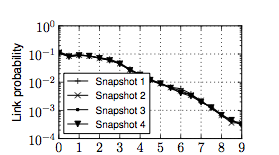
\includegraphics[width=0.8\textwidth]{./Figures/entropy.png}
    \rule{35em}{0.5pt}
  \caption[Probabilit\`{a} di un nuova amicizia rispetto all'entropia di un luogo]{Probabilit\`{a} di un nuova amicizia rispetto all'entropia di un luogo}
  \label{fig:entropy}
\end{figure}



















